\id{ҒТАМР 52.45.19}{}

\begin{articleheader}
{\bfseries НАТРИЙ СУЛЬФИДІНІҢ ҚОСҚҰДЫҚ КЕН ОРЫНДАРЫНЫҢ ТОТЫҚҚАН
ҚОРҒАСЫН-МЫРЫШ КЕНДЕРІНЕ ӘСЕРІН ЗЕРТТЕУ}

{\bfseries
А.Р. Мамбеталиева\textsuperscript{\envelope } \authorid,
А. Мухтаркызы \authorid,
М.Р. Шаутенов} \authorid
\end{articleheader}

\begin{affiliation}
\emph{Satbayev University, Алматы, Казахстан}

\raggedright {\bfseries \textsuperscript{\envelope }}Корреспондент-автор: \href{mailto:a.mambetaliyeva@satbayev.university}{\nolinkurl{a.mambetaliyeva@satbayev.university}}
\end{affiliation}

Тотыққан қорғасын-мырыш кендері өңдеудің күрделілігіне байланысты ұзақ
уақыт бойы толық пайдаланылмады. Бірақ, қорғасын-мырыш сульфидті
кендерінің тез сарқылуына байланысты тотыққан кендерді пайдалану
тиімділігін арттыру қажет. Оксид кендерін алдын-ала байытудың әмбебап
әдістерінің бірі - флотация. Дегенмен, қорғасын-мырыш оксидінің
минералдарының гидрофильдік қасиетінің жоғары болуы, флотация әдісін
қолдануды қиындатады, сонымен қатар мырыш иондарының беткі ерігіштігі,
бұл процестің тиімділігін одан әрі төмендетеді. Бұл қиындықтарды жеңу
үшін сульфидизация әдісінің маңызы жоғыры, ол тотыққан минералдардың
беткі қасиеттерін өзгеретеді және флотацияға дайындайды.

Бұл жұмыста Қосқұдық кен орнының тотыққан кен сынамасындағы қорғасын
минералдарын байыту тиімділігін арттыру мақсатында натрий күкіртін
сульфидизатор ретінде қолданылуына ерекше мән беріледі. Қорғасын алуды
барынша арттыру үшін натрий күкіртінің оңтайлы шығынын анықтау бойынша
зерттеу жүргізілді. Негізгі қорғасын флотациясы кезінде бұл реагенттің
басқа да металлдардың, оның ішінде алтын, күміс және мырыштың, бөлініп
алынуына әсері зерттелді. Зерртеу нәтижесінде натрий күкіртінің шығыны
700 г/т болғанда қорғасынның байыту тиімділігі 10,8\% - ға (34,3-тен
45,1\% - ға дейін) артады. Алынған нәтижелер қорғасын-мырыш
өнеркәсібінің тұрақты дамуын қамтамасыз етудегі өзекті болатын тотыққан
кендерін өңдеу тиімділігін арттыруда негізгі параметрлерін анықтауға
мүмкіндік береді.

{\bfseries Түйін сөздер:} пайдалы қазбаларды байыту, флотация, тотыққан
минералдар, қорғасын, байыту тиімділігі, фазалық талдау, күкіртті
натрий.

\begin{articleheader}
{\bfseries ИССЛЕДОВАНИЕ ВЛИЯНИЯ СУЛЬФИДИРОВАНИЯ С ПРИМЕНЕНИЕМ СЕРНИСТОГО
НАТРИЯ НА ОКИСЛЕННЫЕ СВИНЦОВО-ЦИНКОВЫЕ РУДЫ МЕСТОРОЖДЕНИЯ КОСКУДУК}

{\bfseries
А.Р. Мамбеталиева\textsuperscript{\envelope },
А. Мухтаркызы,
М.Р. Шаутенов}
\end{articleheader}

\begin{affiliation}
\emph{Satbayev University, Алматы, Қазахстан,}

\emph{e-mail: \href{mailto:a.mambetaliyeva@satbayev.university}{\nolinkurl{a.mambetaliyeva@satbayev.university}}}
\end{affiliation}

Окисленные свинцово-цинковые руды долгое время оставались недостаточно
использованными из-за сложности их переработки. Однако в условиях
быстрого истощения запасов свинцово-цинковых сульфидных руд возникает
острая необходимость в повышении эффективности использования этих
оксидных руд. Одним из наиболее универсальных методов предварительного
обогащения оксидных руд является флотация. Однако свинцово-цинковые
оксидные минералы обладают высокой гидрофильностью, что затрудняет их
флотацию, а также они склонны к растворению ионов металлов на
поверхности, что дополнительно снижает эффективность процесса. Для
преодоления этих проблем важную роль играет сульфидизация, которая
позволяет модифицировать поверхностные свойства окисленных минералов,
делая их более пригодными для флотации.

В данной работе особое внимание уделяется влиянию сернистого натрия как
сульфидизатора на эффективность обогащения свинцовых минералов в пробе
окисленной руды с месторождения Коскудук. Было проведено исследование по
определению оптимального расхода сернистого натрия для максимизации
извлечения свинца. Дополнительно анализировалось влияние данного
реагента на извлечение других металлов, таких как золото, серебро и
цинк, в процессе основной свинцовой флотации. Полученные результаты
позволяют определить ключевые параметры для повышения эффективности
переработки оксидных руд, что актуально для обеспечения устойчивого
развития свинцово-цинковой промышленности.

{\bfseries Ключевые слова:} обогащение полезных ископаемых, флотация,
окисленные минералы, свинец, эффективность обогащения, фазовый анализ,
сернистый натрий.

\begin{articleheader}
{\bfseries ON OXIDIZED LEAD-ZINC ORES OF THE KOSKUDUK DEPOSIT INVESTIGATION OF THE EFFECT OF SULFIDATION USING SODIUM SULPHIDE ON OXIDIZED LEAD-ZINC ORES OF THE KOSKUDUK DEPOSIT}

{\bfseries
A.R. Mambetaliyeva\textsuperscript{\envelope },
А. Mukhtarkyzy, M.
Shautenov}
\end{articleheader}

\begin{affiliation}
\emph{Satbayev University, Almaty, Kazakhstan,}

\emph{e-mail:
\href{mailto:a.mambetaliyeva@satbayev.university}{\nolinkurl{a.mambetaliyeva@satbayev.university}}}
\end{affiliation}

Oxidized lead-zinc ores remained underused for a long time due to the
complexity of their processing. However, in conditions of rapid
depletion of reserves of lead-zinc sulfide ores, there is an urgent need
to increase the efficiency of using these oxide ores. One of the most
universal methods of pre-enrichment of oxide ores is flotation. However,
lead-zinc oxide minerals have high hydrophilicity, which makes their
flotation difficult, and they are also prone to dissolution of metal
ions on the surface, which further reduces the efficiency of the
process. To overcome these problems, sulfidization plays an important
role, which makes it possible to modify the surface properties of
oxidized minerals, making them more suitable for flotation.

In this work, special attention is paid to the effect of sodium sulfide
as a sulfidizer on the efficiency of enrichment of lead minerals in a
sample of oxidized ore from the Koskuduk deposit. A study was conducted
to determine the optimal consumption of sodium sulfide to maximize lead
recovery. Additionally, the effect of this reagent on the extraction of
other metals, such as gold, silver and zinc, during the main lead
flotation was analyzed. The results obtained allow us to determine the
key parameters for improving the efficiency of processing oxide ores,
which is important for ensuring the sustainable development of the
lead-zinc industry.

{\bfseries Keywords:} mineral enrichment, flotation, oxidized minerals,
lead, enrichment efficiency, phase analysis, sodium sulfide.

\begin{multicols}{2}
{\bfseries Кіріспе.} Өнеркәсіптік өндірісте мырыш пен қорғасын маңызды
элемент, қорғасын ерекше қасиеттеріне байланысты (жоғары тығыздылығы,
төмен балқу температурасы және жоғары икемділігі) аккумуляторлар,
құрылыс материалдары және радиациядан қорғау жабдықтарын өндіру үшін
шикізат ретінде кеңінен қолданылады. Жоғары беріктігі, тозуға және
коррозияға төзімділігі бар мырыш негізінен металл бұйымдарын және
легирленген материалдар мен құрғақ батареяларды өндіру үшін қолданылады
{[}1{]}.

Құрамында қорғасын-мырыш сульфидтері бар сульфидті кендер ұзақ уақыт
бойы игерілуде, бірақ бай, оңай байытлатын кендер біртіндеп азайуда.
Соңғы жылдары ресурстармен қамтамасыз етудің тенденциясының төмендеуі
байқалуда, бұл өз кезегінде қорғасын мен мырышқа өсіп келе жатқан
сұранысты қанағаттандыру мүмкіндігінің төмендеуіне әкеледі {[}2{]}.
Дегенмен, қорғасын-мырыш кендерінің қоры ауқымды, бірақ олар минералдар
қасиетінің күрделілігімен, ұсақ түйіршікті тау жыныстарының дақтарының
болуымен, еритін тұздардың жоғары болуымен сипатталады, бұл олардың
пайдаланылуын төмендетеді {[}3-6{]}. Сондықтан қорғасын мен мырыш
тотықтарының ресурстарын өндірудің экологиялық тұрғыда таза, тиімді және
үнемді технологияларын құруға бағытталған зерттеулер мен жобалар жүргізу
қажет.

Пайдаланудың қарапайымдылығы, өзіндік құнының төмендігі сияқты
артықшылықтары бар флотация тәсілі -- қорғасын-мырыш кендерін алдын ала
байытудың негізгі әдісі. Минералдардың гидрофильдік қасиетіне байланысты
пайдалы қазбалардың флотациялық әдіспен байытуға әсер ететін негізгі
фактор, қорғасын-мырыш тотыққан минералының бетінің гидрофильділігін
төмендету үшін, әдетте, минералдың бетінде сульфидті қабыршықты
қалыптастыру үшін, сульфидті қайта құру қолданылады, осылайша
флотациялық байытуда тиімділікті арттыру мақсатында минералдың беткі
қасиеттерін өзгертеді {[}7{]}. Сульфидизация әдістеріне негізінен беттік
сульфидизация, күйдіру, механохимиялық және гидротермиялық
сульфидизациялар жатады {[}8, 9{]}. Алайда, сульфидизацияның жоғары
шығындары мен пайдалану қиындықтарына байланысты сульфидті күйдіру,
механохимиялық және гидротермиялық сульфидизация өнеркәсіпте кеңінен
қолданылмайды. Қазіргі уақытта өнеркәсіптік өндіріс негізінен
қорғасын-мырыш тотыққан минералдарының бетін өңдеу үшін күкірт түзетін
агенттерді пайдаланады. Сульфидті өңдеуден кейін тотыққан минералдардың
бетінде пайда болатын сульфидті жұқа қабық борпылдақ және кеуекті
құрылымға ие; ол тотыққан минералдардың гидрофобтылығын күшейте
алғанымен, флотация процесінде кен целлюлозасын араластыру нәтижесінде
пайда болатын ығысу күштерінің әсерінен сульфидті пленка десорбцияға
бейім болады {[}10{]}. Флотациялық реагенттерді қосу тотыққан
минералдардың бетіндегі сульфидизация жылдамдығын тиімді арттырады және
сульфидті жұқа қабықтың бетіндегі механикалық беріктігін жақсартады,
осылайша сульфидті агенттің сульфидтік әсерін күшейтеді {[}11{]}.
Сонымен қатар, бақылау жұмысының дұрыс орындалуы үшін сульфидизациялау
реагентінің мөлшеріне және суспензияның рН деңгейіне аса мән беру қажет
{[}12{]}.

Бұл жұмыста Қосқұдық кен орнының сынамасының заттық құрамының зерттеу
нәтижелері және тоттыққан кендердегі реагенттің беттік флотациялық
қасиетінің ашық тәжірибе нәтижелері ұсынылған.

{\bfseries Материалдар мен әдістер.} Зерттеу нысаны -- Қазақстандағы
Қосқұдық кен орнының тотыққан қорғасын-мырыш кендері.

Қарастырылып отырған кендер мен байыту өнімдерінің заттық құрамы
атомдық-абсорбциялық талдау, атомдық-эмиссиялық талдау, классикалық
химиялық және фотометриялық талдау, талдау жұмыстарын жүргізуге арнайы
дайындалған өкілдік сынамалардағы сынамалық гравиметриялық талдау тобы
әдісімен анықталды.

Минералогиялық сипаттама үшін, орташа сынамалардан басқа, кенді
минералдануы бар негізгі жыныстардың үлгілері таңдалды, олардан мөлдір
тегістеуіштер мен жылтыратылған тегістеуіштер жасалды. Оларды зерттеу
қазіргі заманғы жабдықта физика-химиялық зерттеулер зертханасында
жүргізілді: OLUMPUS BX 51 POL микроскопы., simagis 2R-2C бейнекамерасын
және SIAMS минералды талдауға арналған бағдарламалық жасақтаманы
қолдануымен.

{\bfseries Нәтижелер және талқылау.} Заттық құрамының зерттеу нәтижесінде
қарастырылып отырған тотыққан кеннің сынамасында 0,82 - 0,85\% қорғасын
және 0,6 -- 0,65\% мырыш бар екені анықталды, мыс мөлшері төмен (0,02\%)
және өнеркәсіптік қызығушылық тудырмайды.

Кенде асыл металдардың мөлшері: 0,6 г/т деңгейінде алтын және 5,5 г/т
деңгейінде күміс бар.
\end{multicols}

\begin{table}[H]
\caption*{1 - кесте. Қосқұдық кен орнының тотыққан кенін химиялық фазалық талдау нәтижелері}
\centering
\begin{tblr}{
  row{1} = {c},
  row{2} = {c},
  cell{1}{1} = {r=2}{},
  cell{1}{2} = {c=2}{},
  cell{3}{1} = {c=3}{},
  cell{4}{2} = {c},
  cell{4}{3} = {c},
  cell{5}{2} = {c},
  cell{5}{3} = {c},
  cell{6}{2} = {c},
  cell{6}{3} = {c},
  cell{7}{2} = {c},
  cell{7}{3} = {c},
  cell{8}{2} = {c},
  cell{8}{3} = {c},
  cell{9}{1} = {c=3}{},
  cell{10}{2} = {c},
  cell{10}{3} = {c},
  cell{11}{2} = {c},
  cell{11}{3} = {c},
  cell{12}{2} = {c},
  cell{12}{3} = {c},
  cell{13}{2} = {c},
  cell{13}{3} = {c},
  cell{14}{1} = {c=3}{},
  cell{15}{2} = {c},
  cell{15}{3} = {c},
  cell{16}{2} = {c},
  cell{16}{3} = {c},
  cell{17}{2} = {c},
  cell{17}{3} = {c},
  cell{18}{2} = {c},
  cell{18}{3} = {c},
  vlines,
  hline{1,3-19} = {-}{},
  hline{2} = {2-3}{},
}
{\textbf{Компоненттердің }\\\textbf{атауы}} & \textbf{Құрамы}           &                  \\
                                            & абсолютті, \%             & салыстырмалы, \% \\
Мырыштын бейімделу формасы:                 &                           &                  \\
\textit{- }Суда еритін                      & \textit{\textless{} 0,05} & \textit{-}       \\
\textit{- Тотыққан}                         & \textit{0,25}             & \textit{38,5}    \\
\textit{- Сульфидтер}                       & \textit{0,08}             & \textit{12,3}    \\
\textit{- Ерімейтін}                        & \textit{0,32}             & \textit{49,2}    \\
Жиынтық                                     & 0,65                      & 100,0            \\
Қорғасынның бейімделу формасы:              &                           &                  \\
\textit{- }Құрамында оттегі бар\textit{}    & \textit{0,54}             & \textit{65,8}    \\
\textit{- Галенит}                          & \textit{0,14}             & \textit{17,1}    \\
\textit{- }Қалдық формалар                  & \textit{0,14}             & \textit{17,1}    \\
Жиынтық                                     & 0,82                      & 100,0            \\
Темірдін бейімделу формасы:                 &                           &                  \\
\textit{- Сульфидтер}                       & \textit{\textless{} 0,05} & \textit{-}       \\
\textit{- Екі валентті Fe2+}                & \textit{3,06}             & \textit{48,6}    \\
\textit{- Үш валентті Fe3+}                 & \textit{3,24}             & \textit{51,4}    \\
Жиынтық                                     & 6,30                      & 100,0            
\end{tblr}
\end{table}

1 - кестеде фазалық химиялық талдау нәтижелері көрсетілген және
қарастырылып отырған сынама тотыққан түрге жатады, себебі қорғасын
тотыққан және силикат қосылыстарымен есептегенде салыстырмалы құрамы
82,9\% тең, ал мырыш - 87,7\%. Темір толығымен дерлік тотыққан күйде
екенін атап өтуге болады, өйткені темірдің сульфидті формалары өте аз --
0,05\% (абсолютті құрамы).

\begin{figure}[H]
	\centering
	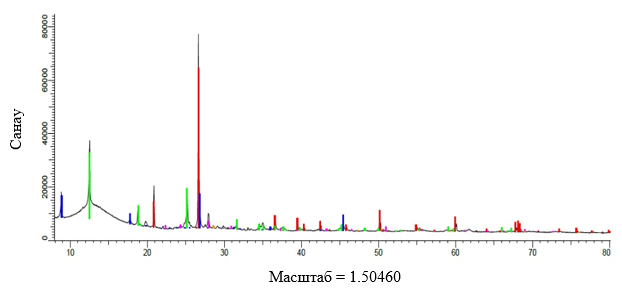
\includegraphics[width=0.9\textwidth]{media/gorn/image6}
	\caption*{1 - сурет. Қосқұдық тотыққан кен сынамасының дифрактограммасы}
\end{figure}

Қарастырылып отырған тотыққан кен сынамасына Bruker (Германия)
D8-ADVANCE дифрактометрінде күрделі минералогиялық құрамына талдаулар
жүргізілді. Қарастырылып отырған кен сынамасының бастапқы
дифрактограммасының нәтижелері 1 -- суретте, 2-кестеде-цифрлық түрде
келтірілген.

\begin{table}
\caption*{2 - кесте. Қосқұдық кен орнының тотыққан кенінің бастапқы сынамасының минералогиялық құрамы}
\centering
\begin{tblr}{
  row{1} = {c},
  cell{2}{2} = {c},
  cell{3}{2} = {c},
  cell{4}{2} = {c},
  cell{5}{2} = {c},
  cell{6}{2} = {c},
  cell{7}{2} = {c},
  cell{8}{2} = {c},
  cell{9}{2} = {c},
  cell{10}{2} = {c},
  cell{11}{2} = {c},
  cell{12}{2} = {c},
  hlines,
  vlines,
}
\textbf{Негізгі минералдар мен комплекстер}              & \textbf{Кендегі құрамы, \%} \\
Қорғасын сульфидтері (галенит)                           & 0,16                        \\
Қорғасынның тотыққан және қалдық түрлері                 & 0,89                        \\
Мырыш сульфидтері (сфалерит)                             & 0,12                        \\
Мырыштын тотыққан және қалдық түрлері                    & 1,07                        \\
Мыс минералдары                                          & 0,04                        \\
Темір сульфидтері (пирит)                                & 0,05                        \\
Темірдің тотыққан түрлері (гетит, гематит)               & 4,51                        \\
Слюда минералдары (альбит, мусковит, клинохлор және тб.) & 53,44                       \\
Кварц                                                    & 30,95                       \\
Басқалары                                                & 8,77                        \\
Барлығы                                                  & 100,00                      
\end{tblr}
\end{table}


Атап өтетін жағдай, кенді және байыту өнімдерін минералогиялық талдауы
гидратталған материалдың жұқа шламдары мен суспензияларының барын және
де сульфидті минералдардың оксидтермен (пирит гетит және гематит) алмасу
процессінің кең таралғанын анықтады, ал қалған сульфидті минералдардың
минералогиялық талдауда анықталағандарының көлемі флотациямен бөліп
алынбайтын көлемде (5 мкм-ден аз).

Тотығу дәрежесі бойынша, құрылымдық-текстуралық сипаттамалары бойынша
және қиылысу мөлшері бойынша қарастырылып отырған тотыққан кендері
Қосқұдық кен орнының байытылуы қиын түрлеріне жатады.

Тотыққан кендердің флотациялық зерттеуі натрий күкіртінің режимін
анықтаудан басталды. 2-суретте өткізілген тәжірибенің сызбасы
көрсетілген. Тәжірибе кезінде алыған нәтижелер 3-кестеде көрсетілген.

{\bfseries 2 - сурет. Натрий күкірттің флотация процесіне әсерін сынау бойынша ашық тәжірибелер сызбасы}

Алынған сынақ тәжірибелерінің нәтижелері негізінде реагенттердің келесі
мөлшері ұсынылады:

- бутил ксантогенаты - 200 г/т;

- көбіктендіргіш (Т-80) -- 60 г/т;

- бутил аэрофлоты -- 60 г/т.

\begin{table}
\caption*{3 - кесте. - Натрий сульфатын қолдана отырып, Қосқұдық (КО) кен орнының тотыққан кенінің бастапқы сынамасын флотациялау бойынша ашық тәжірибелердің нәтижелері}
\centering
\resizebox{\linewidth}{!}{%
\begin{tblr}{
  row{1} = {c},
  row{2} = {c},
  cell{1}{1} = {r=2}{},
  cell{1}{2} = {r=2}{},
  cell{1}{3} = {c=5}{},
  cell{1}{8} = {c=5}{},
  cell{1}{13} = {r=2}{},
  cell{3}{1} = {c=13}{},
  cell{4}{2} = {c},
  cell{4}{3} = {c},
  cell{4}{4} = {c},
  cell{4}{5} = {c},
  cell{4}{6} = {c},
  cell{4}{7} = {c},
  cell{4}{8} = {c},
  cell{4}{9} = {c},
  cell{4}{10} = {c},
  cell{4}{11} = {c},
  cell{4}{12} = {c},
  cell{4}{13} = {r=3}{c},
  cell{5}{2} = {c},
  cell{5}{3} = {c},
  cell{5}{4} = {c},
  cell{5}{5} = {c},
  cell{5}{6} = {c},
  cell{5}{7} = {c},
  cell{5}{8} = {c},
  cell{5}{9} = {c},
  cell{5}{10} = {c},
  cell{5}{11} = {c},
  cell{5}{12} = {c},
  cell{6}{2} = {c},
  cell{6}{3} = {c},
  cell{6}{4} = {c},
  cell{6}{5} = {c},
  cell{6}{6} = {c},
  cell{6}{7} = {c},
  cell{6}{8} = {c},
  cell{6}{9} = {c},
  cell{6}{10} = {c},
  cell{6}{11} = {c},
  cell{6}{12} = {c},
  cell{7}{1} = {c=13}{},
  cell{8}{2} = {c},
  cell{8}{3} = {c},
  cell{8}{4} = {c},
  cell{8}{5} = {c},
  cell{8}{6} = {c},
  cell{8}{7} = {c},
  cell{8}{8} = {c},
  cell{8}{9} = {c},
  cell{8}{10} = {c},
  cell{8}{11} = {c},
  cell{8}{12} = {c},
  cell{8}{13} = {r=3}{c},
  cell{9}{2} = {c},
  cell{9}{3} = {c},
  cell{9}{4} = {c},
  cell{9}{5} = {c},
  cell{9}{6} = {c},
  cell{9}{7} = {c},
  cell{9}{8} = {c},
  cell{9}{9} = {c},
  cell{9}{10} = {c},
  cell{9}{11} = {c},
  cell{9}{12} = {c},
  cell{10}{2} = {c},
  cell{10}{3} = {c},
  cell{10}{4} = {c},
  cell{10}{5} = {c},
  cell{10}{6} = {c},
  cell{10}{7} = {c},
  cell{10}{8} = {c},
  cell{10}{9} = {c},
  cell{10}{10} = {c},
  cell{10}{11} = {c},
  cell{10}{12} = {c},
  cell{11}{1} = {c=13}{},
  cell{12}{2} = {c},
  cell{12}{3} = {c},
  cell{12}{4} = {c},
  cell{12}{5} = {c},
  cell{12}{6} = {c},
  cell{12}{7} = {c},
  cell{12}{8} = {c},
  cell{12}{9} = {c},
  cell{12}{10} = {c},
  cell{12}{11} = {c},
  cell{12}{12} = {c},
  cell{12}{13} = {r=3}{c},
  cell{13}{2} = {c},
  cell{13}{3} = {c},
  cell{13}{4} = {c},
  cell{13}{5} = {c},
  cell{13}{6} = {c},
  cell{13}{7} = {c},
  cell{13}{8} = {c},
  cell{13}{9} = {c},
  cell{13}{10} = {c},
  cell{13}{11} = {c},
  cell{13}{12} = {c},
  cell{14}{2} = {c},
  cell{14}{3} = {c},
  cell{14}{4} = {c},
  cell{14}{5} = {c},
  cell{14}{6} = {c},
  cell{14}{7} = {c},
  cell{14}{8} = {c},
  cell{14}{9} = {c},
  cell{14}{10} = {c},
  cell{14}{11} = {c},
  cell{14}{12} = {c},
  cell{15}{1} = {c=13}{},
  cell{16}{2} = {c},
  cell{16}{3} = {c},
  cell{16}{4} = {c},
  cell{16}{5} = {c},
  cell{16}{6} = {c},
  cell{16}{7} = {c},
  cell{16}{8} = {c},
  cell{16}{9} = {c},
  cell{16}{10} = {c},
  cell{16}{11} = {c},
  cell{16}{12} = {c},
  cell{16}{13} = {r=3}{c},
  cell{17}{2} = {c},
  cell{17}{3} = {c},
  cell{17}{4} = {c},
  cell{17}{5} = {c},
  cell{17}{6} = {c},
  cell{17}{7} = {c},
  cell{17}{8} = {c},
  cell{17}{9} = {c},
  cell{17}{10} = {c},
  cell{17}{11} = {c},
  cell{17}{12} = {c},
  cell{18}{2} = {c},
  cell{18}{3} = {c},
  cell{18}{4} = {c},
  cell{18}{5} = {c},
  cell{18}{6} = {c},
  cell{18}{7} = {c},
  cell{18}{8} = {c},
  cell{18}{9} = {c},
  cell{18}{10} = {c},
  cell{18}{11} = {c},
  cell{18}{12} = {c},
  cell{19}{1} = {c=13}{},
  cell{20}{2} = {c},
  cell{20}{3} = {c},
  cell{20}{4} = {c},
  cell{20}{5} = {c},
  cell{20}{6} = {c},
  cell{20}{7} = {c},
  cell{20}{8} = {c},
  cell{20}{9} = {c},
  cell{20}{10} = {c},
  cell{20}{11} = {c},
  cell{20}{12} = {c},
  cell{20}{13} = {r=3}{c},
  cell{21}{2} = {c},
  cell{21}{3} = {c},
  cell{21}{4} = {c},
  cell{21}{5} = {c},
  cell{21}{6} = {c},
  cell{21}{7} = {c},
  cell{21}{8} = {c},
  cell{21}{9} = {c},
  cell{21}{10} = {c},
  cell{21}{11} = {c},
  cell{21}{12} = {c},
  cell{22}{2} = {c},
  cell{22}{3} = {c},
  cell{22}{4} = {c},
  cell{22}{5} = {c},
  cell{22}{6} = {c},
  cell{22}{7} = {c},
  cell{22}{8} = {c},
  cell{22}{9} = {c},
  cell{22}{10} = {c},
  cell{22}{11} = {c},
  cell{22}{12} = {c},
  cell{23}{1} = {c=13}{},
  cell{24}{2} = {c},
  cell{24}{3} = {c},
  cell{24}{4} = {c},
  cell{24}{5} = {c},
  cell{24}{6} = {c},
  cell{24}{7} = {c},
  cell{24}{8} = {c},
  cell{24}{9} = {c},
  cell{24}{10} = {c},
  cell{24}{11} = {c},
  cell{24}{12} = {c},
  cell{24}{13} = {r=3}{c},
  cell{25}{2} = {c},
  cell{25}{3} = {c},
  cell{25}{4} = {c},
  cell{25}{5} = {c},
  cell{25}{6} = {c},
  cell{25}{7} = {c},
  cell{25}{8} = {c},
  cell{25}{9} = {c},
  cell{25}{10} = {c},
  cell{25}{11} = {c},
  cell{25}{12} = {c},
  cell{26}{2} = {c},
  cell{26}{3} = {c},
  cell{26}{4} = {c},
  cell{26}{5} = {c},
  cell{26}{6} = {c},
  cell{26}{7} = {c},
  cell{26}{8} = {c},
  cell{26}{9} = {c},
  cell{26}{10} = {c},
  cell{26}{11} = {c},
  cell{26}{12} = {c},
  cell{27}{1} = {c=13}{},
  cell{28}{2} = {c},
  cell{28}{3} = {c},
  cell{28}{4} = {c},
  cell{28}{5} = {c},
  cell{28}{6} = {c},
  cell{28}{7} = {c},
  cell{28}{8} = {c},
  cell{28}{9} = {c},
  cell{28}{10} = {c},
  cell{28}{11} = {c},
  cell{28}{12} = {c},
  cell{28}{13} = {r=3}{c},
  cell{29}{2} = {c},
  cell{29}{3} = {c},
  cell{29}{4} = {c},
  cell{29}{5} = {c},
  cell{29}{6} = {c},
  cell{29}{7} = {c},
  cell{29}{8} = {c},
  cell{29}{9} = {c},
  cell{29}{10} = {c},
  cell{29}{11} = {c},
  cell{29}{12} = {c},
  cell{30}{2} = {c},
  cell{30}{3} = {c},
  cell{30}{4} = {c},
  cell{30}{5} = {c},
  cell{30}{6} = {c},
  cell{30}{7} = {c},
  cell{30}{8} = {c},
  cell{30}{9} = {c},
  cell{30}{10} = {c},
  cell{30}{11} = {c},
  cell{30}{12} = {c},
  cell{31}{1} = {c=13}{},
  cell{32}{2} = {c},
  cell{32}{3} = {c},
  cell{32}{4} = {c},
  cell{32}{5} = {c},
  cell{32}{6} = {c},
  cell{32}{7} = {c},
  cell{32}{8} = {c},
  cell{32}{9} = {c},
  cell{32}{10} = {c},
  cell{32}{11} = {c},
  cell{32}{12} = {c},
  cell{32}{13} = {r=3}{c},
  cell{33}{2} = {c},
  cell{33}{3} = {c},
  cell{33}{4} = {c},
  cell{33}{5} = {c},
  cell{33}{6} = {c},
  cell{33}{7} = {c},
  cell{33}{8} = {c},
  cell{33}{9} = {c},
  cell{33}{10} = {c},
  cell{33}{11} = {c},
  cell{33}{12} = {c},
  cell{34}{2} = {c},
  cell{34}{3} = {c},
  cell{34}{4} = {c},
  cell{34}{5} = {c},
  cell{34}{6} = {c},
  cell{34}{7} = {c},
  cell{34}{8} = {c},
  cell{34}{9} = {c},
  cell{34}{10} = {c},
  cell{34}{11} = {c},
  cell{34}{12} = {c},
  cell{35}{1} = {c=13}{},
  cell{36}{2} = {c},
  cell{36}{3} = {c},
  cell{36}{4} = {c},
  cell{36}{5} = {c},
  cell{36}{6} = {c},
  cell{36}{7} = {c},
  cell{36}{8} = {c},
  cell{36}{9} = {c},
  cell{36}{10} = {c},
  cell{36}{11} = {c},
  cell{36}{12} = {c},
  cell{36}{13} = {r=3}{c},
  vlines,
  hline{1,3-4,7-8,11-12,15-16,19-20,23-24,27-28,31-32,35-36,39} = {-}{},
  hline{2} = {3-12}{},
  hline{5-6,9-10,13-14,17-18,21-22,25-26,29-30,33-34,37-38} = {1-12}{},
}
{Өнімдердің\\атауы}            & {Шығуы,\\\%}   & Құрамы, \%    &               &               &               &               & Байыту дережесі &                &                &                &                & {Байыту\\тиімділігі\\eueueu} \\
                               &                & Pb            & Zn            & Au *          & Ag*           & Fe            & Pb              & Zn             & Au             & Ag             & Fe             &                              \\
\textit{«0» тәжірибе; рН-8,68} &                &               &               &               &               &               &                 &                &                &                &                &                              \\
\textit{Концентрат}            & \textit{4,6}   & \textit{4,92} & \textit{1,20} & \textit{7,44} & \textit{60,0} & \textit{6,69} & \textit{26,40}  & \textit{8,80}  & \textit{58,00} & \textit{50,80} & \textit{4,90}  & \textit{21,80}               \\
\textit{Қалдық}                & \textit{95,4}  & \textit{0,66} & \textit{0,60} & \textit{0,26} & \textit{2,80} & \textit{6,28} & \textit{73,60}  & \textit{91,20} & \textit{42,00} & \textit{49,20} & \textit{95,10} &                              \\
\textit{Басты сынама}          & \textit{100,0} & \textit{0,86} & \textit{0,63} & \textit{0,59} & \textit{5,43} & \textit{6,30} & \textit{100,0}  & \textit{100,0} & \textit{100,0} & \textit{100,0} & \textit{100,0} &                              \\
Na2S – 200 г/т; pH – 9,30      &                &               &               &               &               &               &                 &                &                &                &                &                              \\
Концентрат                     & 4,60           & 7,12          & 1,20          & 7,75          & 60,50         & 6,34          & 38,9            & 8,80           & 59,00          & 51,90          & 4,60           & 34,30                        \\
Қалдық                         & 95,40          & 0,54          & 0,60          & 0,26          & 2,70          & 6,30          & 61,10           & 91,20          & 41,00          & 48,10          & 95,40          &                              \\
Басты сынама                   & 100,0          & 0,84          & 0,63          & 0,60          & 5,36          & 6,30          & 100,0           & 100,0          & 100,0          & 100,0          & 100,0          &                              \\
Na2S – 300 г/т; pH – 9,40      &                &               &               &               &               &               &                 &                &                &                &                &                              \\
Концентрат                     & 4,50           & 7,86          & 1,20          & 8,07          & 62,00         & 6,28          & 42,60           & 8,70           & 60,30          & 52,00          & 4,50           & 38,10                        \\
Қалдық                         & 95,50          & 0,50          & 0,59          & 0,25          & 2,70          & 6,30          & 57,4            & 91,30          & 39,70          & 48,00          & 95,50          &                              \\
Басты сынама                   & 100,0          & 0,83          & 0,62          & 0,60          & 5,37          & 6,30          & 100,0           & 100,0          & 100,0          & 100,0          & 100,0          &                              \\
Na2S – 400 г/т; pH – 9,57      &                &               &               &               &               &               &                 &                &                &                &                &                              \\
Концентрат                     & 4,40           & 8,52          & 1,20          & 8,22          & 68,20         & 6,24          & 45,00           & 8,60           & 61,20          & 55,70          & 4,40           & 40,60                        \\
Қалдық                         & 95,60          & 0,48          & 0,59          & 0,24          & 2,50          & 6,30          & 55,00           & 91,40          & 38,80          & 44,30          & 95,60          &                              \\
Басты сынама                   & 100,0          & 0,83          & 0,62          & 0,59          & 5,39          & 6,30          & 100,0           & 100,0          & 100,0          & 100,0          & 100,0          &                              \\
Na2S – 500 г/т; pH – 9,61      &                &               &               &               &               &               &                 &                &                &                &                &                              \\
Концентрат                     & 3,10           & 13,0          & 1,48          & 12,6          & 112,9         & 6,20          & 46,90           & 7,40           & 65,80          & 65,50          & 3,10           & 43,80                        \\
Қалдық                         & 96,90          & 0,47          & 0,59          & 0,21          & 1,90          & 6,30          & 53,10           & 92,60          & 34,20          & 34,50          & 96,9           &                              \\
Басты сынама                   & 100,0          & 0,86          & 0,62          & 0,59          & 5,34          & 6,30          & 100,0           & 100,0          & 100,0          & 100,0          & 100,0          &                              \\
Na2S – 700 г/т; pH – 9,81      &                &               &               &               &               &               &                 &                &                &                &                &                              \\
Концентрат                     & 3,10           & 13,4          & 1,40          & 11,1          & 103,9         & 5,96          & 48,2            & 7,10           & 59,60          & 60,20          & 2,90           & 45,10                        \\
Қалдық                         & 96,90          & 0,46          & 0,59          & 0,24          & 2,20          & 6,31          & 51,80           & 92,90          & 40,40          & 39,80          & 97,10          &                              \\
Басты сынама                   & 100,0          & 0,86          & 0,62          & 0,58          & 5,35          & 6,30          & 100,0           & 100,0          & 100,0          & 100,0          & 100,0          &                              \\
Na2S – 1000 г/т; pH – 10,41    &                &               &               &               &               &               &                 &                &                &                &                &                              \\
Концентрат                     & 3,90           & 9,86          & 1,17          & 9,29          & 80,10         & 5,94          & 45,50           & 7,40           & 58,30          & 57,50          & 3,70           & 41,60                        \\
Қалдық                         & 96,10          & 0,48          & 0,59          & 0,27          & 2,40          & 6,31          & 54,50           & 92,60          & 41,70          & 42,50          & 96,30          &                              \\
Басты сынама                   & 100,0          & 0,85          & 0,61          & 0,62          & 5,43          & 6,30          & 100,0           & 100,0          & 100,0          & 100,0          & 100,0          &                              \\
Na2S – 1500 г/т; pH – 10,86    &                &               &               &               &               &               &                 &                &                &                &                &                              \\
Концентрат                     & 9,00           & 3,50          & 0,69          & 2,31          & 23,30         & 6,14          & 37,40           & 10,20          & 34,70          & 39,00          & 8,80           & 28,40                        \\
Қалдық                         & 91,00          & 0,58          & 0,60          & 0,43          & 3,60          & 6,30          & 62,60           & 89,80          & 65,30          & 61,00          & 91,20          &                              \\
Басты сынама                   & 100,0          & 0,84          & 0,61          & 0,60          & 5,37          & 6,29          & 100,0           & 100,0          & 100,0          & 100,0          & 100,0          &                              \\
Na2S – 2000 г/т; pH – 11,50    &                &               &               &               &               &               &                 &                &                &                &                &                              \\
Концентрат                     & 12,10          & 1,85          & 0,64          & 1,10          & 12,40         & 6,32          & 26,40           & 12,80          & 22,60          & 28,00          & 12,10          & 14,30                        \\
Қалдық                         & 87,90          & 0,71          & 0,60          & 0,52          & 4,40          & 6,30          & 73,60           & 87,20          & 77,40          & 72,00          & 87,90          &                              \\
Басты сынама                   & 100,0          & 0,85          & 0,60          & 0,59          & 5,37          & 6,30          & 100,0           & 100,0          & 100,0          & 100,0          & 100,0          &                              
\end{tblr}
}
\end{table}

\begin{figure}[H]
	\centering
	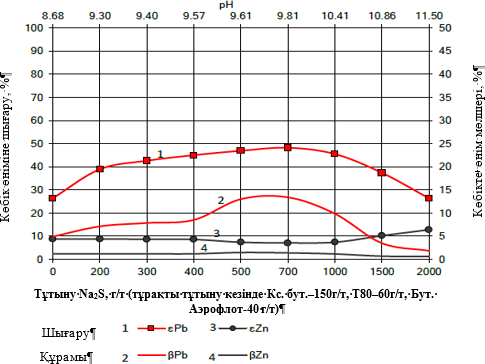
\includegraphics[width=0.6\textwidth]{media/gorn/image7}
	\caption*{2 - сурет. Натрий күкірттің мөлшері Қосқұдық кен орнының тотыққан кенінің бастапқы сынамасының Pb және Zn флотация көрсеткіштеріне әсері}
\end{figure}

\begin{figure}[H]
	\centering
	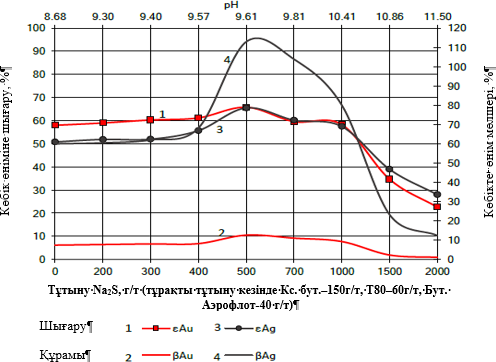
\includegraphics[width=0.6\textwidth]{media/gorn/image8}
	\caption*{3 - сурет. Натрий күкіртінің мөлшері Қосқұдық кен орнының тотыққан кенінің бастапқы сынамасының Au және Ag флотация көрсеткіштеріне әсері}
\end{figure}

\begin{multicols}{2}
3-суреттегі мәліметтерден натрий күкірттінің шығыны 200 г/т -- ден 700
г/т-ға дейін артқан сайын қорғасынның байыту тиімділігі 10,8\% - ға
(34,3-тен 45,1\% - ға дейін) артады, бұл ретте күміс пен алтынның байыту
тиімділігі 60,2 және 59,6\% -ға тең. Асыл металдар үшін натрий
күкіртінің оңтайлы шығыны 500 г/т, күмістің байыту дәрежесі -- 65,5 \%,
алтынның -- 65,8\%-ды көрсетті. Айта кету керек, сульфидизация мырыштың
байыту көрсеткіштерін арттырмайды.

{\bfseries Қорытынды.} Зерттеу Қосқұдық кен орнының тотыққан кенімен
жүргізілді. Заттық құрамы бойынша орташа қорғасын мөлшері -- 0,82 -
0,85\%, мырыш -- 0,6 -- 0,65 \%, күміс -- 5,5 г/т және алтын -- 0,6 г/т
тең, мыс мөлшері - 0,02\% және өнеркәсіптік қызығушылық тудырмайды.

Фазалық талдау нәтижесіне сәйкес, сынама тотыққан қосылыстарға жатады,
себебі қорғасынның, тотыққан және силикат қосылыстарымен есептегенде,
салыстырмалы құрамы 82,9\% тең, ал мырыш - 87,7\%.

Қосқұдық кен орнының тотыққан кендерін байыту кезінде негізгі
реагенттердің шығындары анықталды: бутил ксантогенаты -- 200 г/т; көбік
түзуші (Т-80) -- 60 г/т; бутил аэрофлоты -- 60 г/т. Негізгі, бақылау
флотациясының уақыты -- 10 минут және 6 минутты құрады.

Ашық сынақ тәжірибелерінің нәтижесінде натрий күкіртінің шығыны шамамен
700 г/т болған кезде қорғасынның тиімділігі артады, ал күміс пен алтын
үшін шамамен 500 г/т тең. Айта кету керек, сульфидизация мырыштың байыту
көрсеткіштерін арттырмайды.

\emph{{\bfseries Қаржыландыру.} Жұмыс Қазақстан Республикасы Білім және
Ғылым министрлігінің ғылым комитеті қаржыландыратын АР 23489765 гранттық
жобасы бойынша орындалды.}
\end{multicols}

\begin{center}
{\bfseries References}
\end{center}

\begin{references}
1. Nayak A., Jena M.S., Mandre N.R., Beneficiation of Lead-Zinc Ores -- A
// Review. Mineral Processing and Extractive Metallurgy Review.
-2021.-Vol.43(5). -P. 564 - 583. DOI 10.1080/08827508.2021.1903459

2. Gavin M.M., Simon M. J., Timothy T.W. The world' s
lead-zinc mineral resources: Scarcity, data, issues and opportunities
//
\href{https://www.sciencedirect.com/journal/ore-geology-reviews}{Ore
Geology Reviews}. -2017.
-\href{file:///C:/Users/admin/Desktop/Вестник\%20КазУТБ/Vol.\%2080}{Vol.
80}. -P. 1160-1190

DOI 10.1016/j.oregeorev.2016.08.010

3. Abkhoshk E., Jorjani E., Al-Harahsheh M.S., Rashchi F., Naazeri M.,
Review of the hydrometallurgical processing of non-sulfide zinc ores
// Hydrometallurgy. -2014. - Vol.149. - P.153-167. DOI

10.1016/j.hydromet.2014.08.001

4. Liu W.G., Zhao L., Liu W.B., Zheng Y.X., Huang L.Y., Mao Y., Ding
S.Y., Enhanced flotation of smithsonite from calcite based on the
synergistic action of carboxylated chitosan and sodium carbonate //
Adv. Powder Technol. -2023. -Vol. 34 (12):104261

DOI 10.1016/j.apt.2023.104261

5.Mehdilo A., Irannajad M., Zarei H., Flotation of zinc oxide ore using
cationic and cationic-anionic mixed collectors // Physicochem. Probl.
Miner. Process. -2013.-Vol. 49(1). -P. 145−156. DOI
\href{http://dx.doi.org/10.5277/ppmp130114}{10.5277/ppmp130114}

6. Maghfouri S., Hosseinzadeh M.R., Rajabi A., Choulet F., A review of
major non-sulfide zinc deposits in Iran // Geosci. Front. -2018. --Vol.
9(1). -P.249-272. DOI
\href{https://doi.org/10.1016/j.gsf.2017.04.003}{10.1016/j.gsf.2017.04.003}

7. Yi Y.H., Peixuan Li, Zhang G., Feng Q.C., Han G., Stepwise activation
of hemimorphite surfaces with lead ions and its contribution to
sulfidization flotation // Sep. Purif. Technol. - 2022. --Vol. 299:
121679 DOI
\href{https://doi.org/10.1016/j.seppur.2022.121679}{10.1016/j.seppur.2022.121679}

8. Elizondo-Álvarez M.A., Uribe-Salas A., Nava-Alonso F., Flotation
studies of galena (PbS), cerussite (PbCO\textsubscript{3}) and anglesite
(PbSO\textsubscript{4}) with hydroxamic acids as collectors // Miner.
Eng. -2020. - Vol. 155: 106456
\href{https://doi.org/10.1016/j.mineng.2020.106456}{DOI
10.1016/j.mineng.2020.106456}

9. Xue J.W., Qu Y.B., Chen Y., Zhang C.H., Bu X.Z., Effective sulfide
flotation of cerussite by using trithiocyanuric acid as a novel
sulfurizing reagent // Miner. Eng. -2023.-Vol. 198: 108087

\href{https://doi.org/10.1016/j.mineng.2023.108087}{DOI
10.1016/j.mineng.2023.108087}

10. Zhang S., Xian Y.J., Wen S.M., Liang G.Y., Enhancement of xanthate
adsorption on lead-modified and sulfurized smithsonite surface in the
presence of ammonia // Miner. Eng. -2022. -Vol. 189: 107872 DOI
10.1016/j.mineng.2022.107872

11. Li. Jialei; Pei Bin, Liu Zhicheng; Gao Xiang; Ning Shuai; Cai Zi,
Liu Ruizeng, Applying the surface differences in the sulfophilic and
oxyphilic affinities for reverse flotation separation of calcite from
smithsonite // \href{javascript:void(0)}{Surfaces and Interfaces}.
-2023. - Vol. 42: 103310

DOI 10.1016/j.surfin.2023.103310

12.Qian Wei, Liuyang Dong, Wenqing Qin, Fen Jiao, Zhongxu Qi, Cheng
Feng, Dayong Sun, Long Wang, Shunyuan Xiao, Efficient flotation recovery
of lead and zinc from refractory lead-zinc ores under low alkaline
conditions //
\href{https://www.sciencedirect.com/journal/geochemistry}{Geochemistry}.
-2021.
-\href{https://www.sciencedirect.com/journal/geochemistry/vol/81/issue/4}{Vol.
81.(4}): 125769

DOI 10.1016/j.chemer.2021.125769
\end{references}

\begin{authorinfo}
\emph{{\bfseries Авторлар туралы мәліметтер}}

Мамбеталиева А.Р. - PhD докторы, "Металлургия және пайдалы қазбаларды
байыту" кафедрасының аға оқытушысы Satbayev University, Алматы,
Қазақстан, e-mail:
\href{mailto:a.mambetaliyeva@satbayev.university}{\nolinkurl{a.mambetaliyeva@satbayev.university}};

Мұұхтарқызы А. - "Металлургия және пайдалы қазбаларды байыту"
кафедрасының магистранты Satbayev University, Алматы, Қазақстан, e-mail:
\href{mailto:asel.muktarkyzy@mail.ru}{\nolinkurl{asel.muktarkyzy@mail.ru}};

Шаутенов М.Р. - техникалық ғылымдар кандидаты, доцент, "Металлургия және
пайдалы қазбаларды байыту" кафедрасының профессоры Satbayev University,
Алматы, Қазақстан, e-mail: m.shautenov@satbayev.universit

\emph{{\bfseries Information about the authors}}

Mambetaliyeva A.R. - PhD, Senior Lecturer at the Department of
Metallurgy and Mineral Processing at Satbayev University, Almaty,
Kazakhstan, e-mail:
\href{mailto:a.mambetaliyeva@satbayev.university}{\nolinkurl{a.mambetaliyeva@satbayev.university}};

Mukhtarkyzy A. - Master at the Department of Metallurgy and Mineral
Processing at Satbayev University, Almaty, Kazakhstan, e-mail:
\href{mailto:asel.muktarkyzy@mail.ru}{\nolinkurl{asel.muktarkyzy@mail.ru}};

Shautenov M., Candidate of technical sciences, Professor at the
Department of Metallurgy and Mineral Processing at Satbayev University,
Almaty, Kazakhstan, e-mail:
\href{mailto:m.shautenov@satbayev.university}{\nolinkurl{m.shautenov@satbayev.university}},
\end{authorinfo}
